\title{Concurrency and Parallel Programming \\ Assignment 1}
\author{David van Erkelens and Jelte Fennema \\ Department of Computer Science
    \\ University of Amsterdam} \date{\today}
\documentclass[12pt]{article}
\usepackage{graphicx}
\usepackage{color}
\begin{document}
\maketitle
\section{Assignment 1.1}

As can be seen in the graph, the speedup differs a lot between the different
problem sizes. With the smallest problem size, i\_max = $10^3$, the speedup
with all amount of threads is lower than one. This means that using the
sequential algorithm  is the fastest is this specific case. This is probably
caused by the relatively high amount of time that is spent in the critical
section with small problem sizes. With i\_max = $10^4$ the maximum speedup is at
two threads. After that it goes downhill quickly. \\
The three largest problem sizes all benefit from more threads. The most likely
reason for this is that waiting in a critical section occurs less per
calculations a thread does.\ i\_max = $10^6$ has the largest speedup. With eight
threads it reaches a speedup of a little above five.

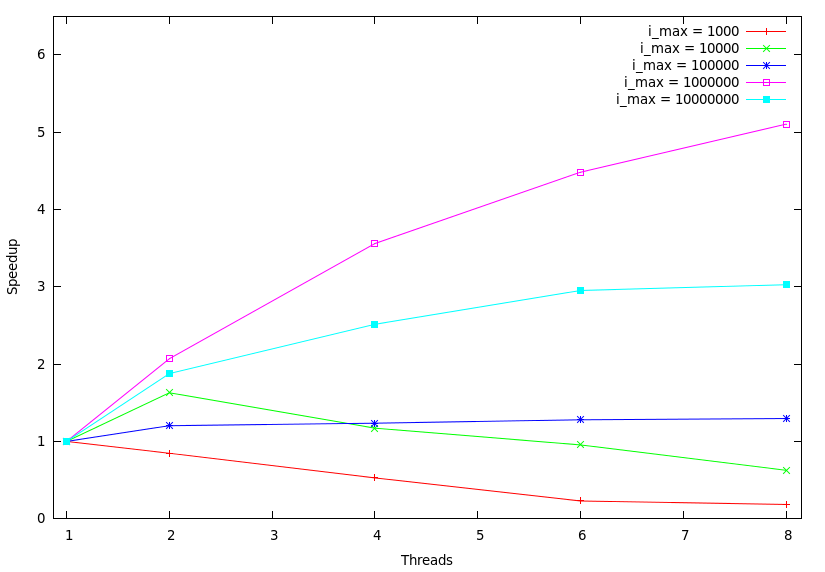
\includegraphics[width=\textwidth]{speedupgraph.png}

\section{Assignment 1.2}
Assignment 1.2 is a program generating an infinite stream of prime numbers,
using the sieve of Eratosthenes. When the program is executed, one main tread
is created. This main thread generates a stream of natural numbers, which are
passed to the next thread. This thread takes the first number of this stream,
which is a 2 for the first "slave-thread". For a slave thread, there are three
options: the number which will be processed is the first number that enters the
thread, which means it is a prime number. This number will then be printed and
the next number will be processed. If the next number can be divided trough the
prime number, it is discarded. When it can't be divided, the number is possibly
a prime number and it will be passed to the next thread. \\ \\
All thread communicate with each other trough a buffer, locked with mutexes to
prevent errors. To ensure all printing will be done, after printing each prime
the stdout buffer will be flushed.
\end {document}
